\graphicspath{{./figures/chapter3/}}
\lstset{inputpath = ../MATLAB}
\pgfplotstableset{search path = ./tables/chapter3}

\chapter{Finite volume method} \label{ch:FVM}

The Finite Volume Method (FVM) is one of the most important discretization
techniques for the numerical solution of partial differential equations,
especially in the context of fluid dynamics and hyperbolic systems
of conservation laws. In the last decades, plenty of effective numerical
schemes have been developed based on this technique; despite their
differences, they all share the same fundamental ideas, which we can
summarize as follows.

First, the spatial domain $\Omega$ of the partial differential equation
is partitioned into a finite number of mutually disjoint \emph{cells},
also known as \emph{control volumes} when $\Omega \subset \R^3$,
and the strong form of the equation is integrated over each of these cells.
Second, the divergence theorem is used to turn the volume integral
over each cell into a boundary integral. In this way, a notion of \emph{flux}
can be meaningfully defined on the boundary of the cells.
Third, the partial differential equation is reduced to either a system
of ordinary differential equations or a system of algebraic equations
by discretizing the boundary integrals and balancing the fluxes
across every pair of neighboring cells. Systems of ordinary differential
equations are obtained from time-dependent problems, since the finite
volume method only discretizes the spatial part of the partial differential
equation. This semidiscretization process is known as \emph{method of lines},
and allows us to simplify our numerical schemes by decoupling the spatial
discretization from the temporal one.

In this work we focus on cell-averaged finite volume methods for initial
boundary value problems given by the compressible Euler equations and,
more generally, any hyperbolic system of conservation laws.
The adjective \emph{cell-averaged} means that the unknowns in the resulting
system of ordinary differential equations are the integral means
\[
\bar{\vec{u}}_i(t) = \frac{1}{\abs{C_i}} \int_{C_i} \vec{u}(\vec{x},t) \dx
\qquad \text{$i = 1,\dots,N_c$}
\]
of the solution $\vec{u}(\vec{x},t)$ over each cell $C_i$, with
$N_c$ total number of cells.
This is unlike other families of finite volume schemes,
like \emph{cell-centered} and \emph{cell-vertex} schemes, which instead
associate the unknowns to pointwise values of the solution
$\vec{u}(\vec{x},t)$ at the center of the cells or at their vertices, respectively.

The finite volume method dates back to the mid-60s, when it was independently
introduced by multiple researchers working in the field of computational
fluid dynamics as a way to overcome some of the limitations of classical
finite difference schemes that were in use at the time, most notably the
lack of exact conservation of physical quantities such as mass, momentum
or energy at the discrete level \cite{runchal2013emergence}
\cite{mcdonald1971computation} \cite{maccormack1972computational}.

As a rule of thumb, finite volume methods compare favorably to other
discretization techniques in terms of qualitative properties of the solutions,
like conservation and monotonicity, but are somewhat lacking in the
quantitative aspects.
To be more precise, let~$e(h)$ be the worst-case error in the spatial
discretization given by a finite volume scheme as a function of a parameter
$h$ that determines how fine the partition of $\Omega$ is (for instance,
$h$ could be an upper bound on the diameter of every cell of the partition).
If $e(h) = O(h^K)$ for some $K > 0$, then we say that the finite volume scheme
has (at least) order $K$. The supremum of all $K$ such that $e(h) = O(h^K)$
is known as \emph{the} order of the scheme.
All else being equal, a scheme of high order is preferred over a scheme
of low order, because a coarser grid can be used to achieve the same
error target on the solution: this means that high-order schemes are more
computationally efficient, at least in an asymptotic sense.

Finite volume methods of order higher than two are not straightforward
to define, because most classical methods approximate pointwise values
of the solution $\vec{u}(\vec{x},t)$ in a cell $C_i$ with the cell-average
$\bar{\vec{u}}_i(t)$ and then freely switch back and forth between the two;
this approximation is at best $O(h^2)$ accurate at the barycenter of each cell,
however, and~$O(h^1)$ accurate everywhere else, so high-order schemes require
a different approach.

To be fair, low orders of convergence are rarely seen as a serious
drawback of classical finite volume schemes, because in computational
fluid dynamics the emphasis is usually on capturing the correct qualitative
aspects of the flow, rather than trying to get as close as possible to the
exact solution in a quantitative sense (as the latter task can be 
prohibitively expensive in terms of computations).
Nevertheless, in recent years the interest towards high order
methods for fluid dynamics and advection-dominated problems
has grown considerably, and it is conceivable that in the future
high-order schemes will become more widespread in both academia and industry.
For a review article on the adoption of high-order methods in computational
fluid dynamics, we refer to \cite{vincent2011facilitating}.

The rest of this chapter is structured as follows. In the first four sections
we define in detail the LLS-$K$ family of finite volume schemes on polygonal
meshes and prove that they have arbitrarily high order $K$.
Section \ref{sec:boundary-condtions} covers the numerical treatment
of boundary conditions for the Euler equations.
In Section \ref{sec:mesh-generation} we explain how high-quality polygonal
meshes can be generated from a sequence of pseudorandom points in 2D
and a description of $\partial \Omega$.
In Section \ref{sec:temporal-discretization} we introduce the SSP family
of Runge-Kutta schemes for the temporal discretization of the system
of ordinary differential equations that is produced by the finite volume method.
In Section \ref{sec:numerical-tests-smooth} we compare the results given
by our numerical schemes with two smooth closed-form solutions of the Euler equations:
a traveling wave and an isentropic vortex. The rates of convergence
of the errors in various norms confirm the effectiveness of our numerical schemes.

\section{Spatial discretization} \label{sec:spatial-discretization}

Let us now see the details of how the LLS-$K$ family of finite
volume schemes is defined. Let us consider an initial boundary
value problem for a hyperbolic system of conservation laws
with generic boundary conditions
\begin{equation} \label{generic_IVBP}
\begin{cases}
\partial_{t} \vec{u}(\vec{x},t) + \diver(\tns{F}(\vec{u}(\vec{x},t))) = 0,
	\qquad \vec{x} \in \Omega, \; t \in [0,T], \\
\vec{u}(\vec{x},0) = \vec{u}_{0}(\vec{x}) \text{ in $\Omega$}, \\
\text{Boundary conditions on $\partial\Omega\times [0,T]$}.
\end{cases}
\end{equation}	
We did not specify boundary conditions because their numerical
treatment requires ad hoc techniques that we postpone to
Section \ref{sec:boundary-condtions}.
For the time being, we can focus on the definition of finite
volume methods in the interior of the domain only.
	
Suppose that the domain $\Omega$ has piecewise linear boundary.
If that is not the case (e.g.\ $\Omega$ is a circle), then we can first
approximate its boundary with piecewise linear closed simple curves
such that the resulting perturbation on the exact solution is arbitrarily
small (this is always possible, as long as the initial boundary value
problem is well-posed with respect to $\partial\Omega$ and the piecewise
boundaries converge to $\partial\Omega$ in a sufficiently regular way).

Further, let us suppose that $\Omega$ has been partitioned into a
finite number $N_{c}$ of disjoint nonempty convex simple polygons
$\{C_{i} \mid i=1,\dots, N_{c}\}$. Such a partition is also known as
\emph{tessellation} of $\Omega$, or \emph{mesh}.
Let $d_{i}$ be the indiameter of $C_{i}$, that is, the diameter of the
greatest circle entirely contained within $C_{i}$.
The quantity $d_{i}$ is not easy to compute exactly for an arbitrary
convex polygon. For this reason, we propose the following
approximation of $d_{i}$:
\begin{equation} \label{eq:definition-h}
h_{i} = \frac{4 \cdot \text{Area}(C_{i})}{\text{Perimeter}(C_{i})}
\end{equation}
The rationale behind this choice is that $h_{i} = d_{i}$ for important subclasses
of convex polygons, like triangles or regular polygons, and that even
when $h_{i} \neq d_{i}$ the following inequality still holds
\cite{scott2000inequalities}:
\[
\frac{1}{2}h_{i}\leq d_{i} \leq h_{i}.
\]
Let $h$ be the maximum value of $h_{i}$ on any
given polygonal partition of $\Omega$.
Whenever we talk about numerical methods with \emph{order} $K$,
we are are implicitly working under the assumption
that a family $\mathcal{F}$ of increasingly fine partitions $\mathcal{T}_{h}$
has been defined, and that the error $e(h)$ goes to zero like $O(h^K)$
as $h \to 0$, i.e.\ as the partitions get finer and finer.

Naturally, the error $e(\cdot)$ is not \emph{really} a function of $h$:
the error depends on the choice of the family $\mathcal{F}$,
so for a fixed $h > 0$ we could define two different tessellations
$\mathcal{T}_{h}^1$ and $\mathcal{T}_{h}^2$ such that
\[
h_i < h \text{ for each $C_i \in \mathcal{T}_{h}^1$}
\qquad \text{and} \qquad
h_\ell < h \text{ for each $C_\ell \in \mathcal{T}_{h}^2$},
\]
and there is no reason to expect $e(\mathcal{T}_{h}^1)$ to be
exactly equal to $e(\mathcal{T}_{h}^2)$.
Nevertheless, in the field of numerical analysis it is typically
possible to prove that, under some regularity assumptions on the
shrinking process of the tessellations, there exists a number $K \geq 0$
such that $e(\mathcal{T}_{h}) = O(h^K)$ for all (regular) families
$\mathcal{F}$. Depending on the numerical method and the proof technique,
$h$ may not be defined as in \eqref{eq:definition-h}
(for example, it could be the maximum among the diameters of every cell),
but the point still stands: if we are only interested in the asymptotic
behavior of $e(\cdot)$, for nice families of tessellations we can think
of the error as a function of $h$ instead of $\mathcal{T}_{h}$.

What makes a family of tessellations \emph{nice} is hard to say in
general, though, as it heavily depends on the definition of the
numerical scheme that is used to approximate the solution to
the partial differential equation. The following are two common assumptions:

\begin{defi}[Shape-regularity] \label{defi:shape-regularity}
A family of tessellations $\mathcal{F}$ is \emph{shape-regular}
if there exists a constant $\delta > 0$ independent of $h$ such that
\[
\text{Diameter}(C_i) \leq \delta h_i
\quad \text{for all $C_i \in \mathcal{T}_{h}$
and for all $\mathcal{T}_{h} \in \mathcal{F}$}.
\]
\end{defi}

\begin{defi}[Quasi-uniformity]
A family of tessellations $\mathcal{F}$ is \emph{quasi-uniform}
if there exists a constant $\tau \geq 1$ independent of $h$ such that
\[
h \leq \tau h_i
\quad \text{for all $C_i \in \mathcal{T}_{h}$
and for all $\mathcal{T}_{h} \in \mathcal{F}$}.
\]
\end{defi}

As explained in the previous section, cell-averaged finite volume methods
reduce a system of partial differential equations like \eqref{generic_IVBP}
to a system of ordinary differential equations whose unknowns are the cell averages
\[
\bar{\vec{u}}_{i}(t)=\frac{1}{\abs{C_{i}}} \int_{C_{i}} \vec{u}(\vec{x},t) \dx,
\]
with $\abs{C_{i}} = \text{Area}(C_{i})$. By the definition of hyperbolic system
of conservation laws and by the divergence theorem, we compute %that
\begin{equation} \label{FVM_divergence}
\begin{aligned}
\partial_{t} \bar{\vec{u}}_{i}(t)
&= \frac{1}{\abs{C_i}} \int_{C_{i}} \partial_{t} \vec{u}(\vec{x},t) \dx
 = \frac{1}{\abs{C_i}} \int_{C_{i}} -\diver(\tns{F}(\vec{u}(\vec{x},t))) \dx \\
&= -\frac{1}{\abs{C_i}} \int_{\partial C_{i}}
	\tns{F}(\vec{u}(\vec{x},t)) \cdot \vec{\nu}(\vec{x}) \dsigma.
\end{aligned}
\end{equation}
Since $C_{i}$ is a polygon, its boundary can be written as a disjoint union
of $N_{e}(i)$ oriented segments, its edges:
\[
\partial C_{i}=\bigcup_{j=1}^{N_{e}(i)} \Gamma_{ij}.
\]
Without loss of generality, we can always assume that, whenever two cells
share more than a vertex, they share the same edge (we call them
\emph{neighboring cells}).
This is because vertices on the boundary of each polygon can be freely
added or removed to satisfy this constraint,
without modifying the actual shape of the cell.
A polygonal tessellation that satisfies this constraint is called
\emph{conforming}; a vertex that violates conformity is known as
\emph{hanging node}. Finite volume methods can only be defined on
conforming tessellations.

Let $\{\vec{\nu}_{ij}\}$ be an arbitrary but coherent way to
define normals all over a mesh. This means that, whenever two cells
$C_{i}$ and $C_{\hat{i}}$ share an edge $\Gamma_{ij}=\Gamma_{\hat{i}\hat{j}}$,
we must have $\vec{\nu}_{ij}=\vec{\nu}_{\hat{i}\hat{j}}$.
Since the divergence theorem requires $\vec{\nu}(\vec{x})$ to point away
from $C_{i}$, on some cells we may have $\vec{\nu}(\vec{x}) = \vec{\nu}_{ij}$,
and on the other cells we may have $\vec{\nu}(\vec{x}) = -\vec{\nu}_{ij}$.
We therefore introduce the \emph{normal sign} function $s_{ij}$ such that
$\vec{\nu}(\vec{x}) = s_{ij} \vec{\nu}_{ij}$ on $\Gamma_{ij}$.
Equation \eqref{FVM_divergence} becomes
\[
\partial_{t}\bar{\vec{u}}_{i}(t)
= -\frac{1}{\left|C_{i}\right|} \sum_{j=1}^{N_{e}(i)} \int_{\Gamma_{ij}}
	\tns{F}(\vec{u}(\vec{x},t)) \cdot s_{ij} \vec{\nu}_{ij} \dsigma.
\]
The integral over each edge can then be discretized by a quadrature
formula. Let $N_q$ be the number of nodes in the quadrature formula,
let $w_{k}$ be its weights and let $\tau_{k}$ be its quadrature nodes,
normalized in the $[0,1]$ interval instead of the more common $[-1,1]$.
Furthermore, let $\vec{v}_{ij1}$, $\vec{v}_{ij2}$ be the endpoints of $\Gamma_{ij}$,
coherently defined all over the mesh such that the vector
$\vec{v}_{ij1}-\vec{v}_{ij2}$, when normalized, is the $90$ degrees
counterclockwise rotation of $\vec{\nu}_{ij}$.
By introducing the quadrature points
$\vec{x}_{ijk} = (1-\tau_{k}) \vec{v}_{ij1} + \tau_{k} \vec{v}_{ij2}$, we get 
\[
\partial_{t}\bar{\vec{u}}_{i}(t)
\approx -\frac{1}{\left|C_{i}\right|}\sum_{j=1}^{N_{e}(i)} \abs{\Gamma_{ij}}
\sum_{k=1}^{N_{q}} w_{k} \tns{F}(\vec{u}(\vec{x}_{ijk},t)) \cdot s_{ij}\vec{\nu}_{ij}.
\]
All that is left to do now is choosing a way to \emph{reconstruct} the values
of $\vec{u}(\vec{x}_{ijk},t)$ from the cell-averaged values $\bar{\vec{u}}_{i}(t)$
or, more precisely, to reconstruct the normal
fluxes $\tns{F}(\vec{u}(\vec{x}_{ijk},t)) \cdot \vec{\nu}_{ij}$
(as evaluating $\tns{F}$ in $\vec{u}(\vec{x}_{ijk},t)$ is not the only way to do so).
Since we need to handle both smooth and discontinuous solutions
$\vec{u}(\vec{x},t)$, this is not a simple task.
The standard approach here is to introduce Godunov's method.

\section{Godunov's method} \label{sec:godunov-method}
Godunov's method is a way to approximate the fluxes
$\tns{F}(\vec{u}(\vec{x}_{ijk},t))$ on each edge by solving
an exact or approximate Riemann problem at each inter-cell boundary.
The method takes its name from the Russian mathematician Sergei K.\ Godunov,
who first introduced this method for one-dimensional domains in 1959.
In the more general $n$-dimensional setting, the method works in the
following way.

First, reconstructions $\vec{u}^{+}_{ijk}(t)$ and $\vec{u}^{-}_{ijk}(t)$
are defined on opposite sides of each edge by the formula
\begin{equation} \label{reconstruction-strategy}
\begin{cases}
\vec{u}^{+}_{ijk}(t) = \bar{\vec{u}}_{i}(t) \text{ for all }k=1,\dots,N_{q}
	&\text{if }\vec{\nu}_{ij} \text{ points into } C_i, \\
\vec{u}^{-}_{ijk}(t) = \bar{\vec{u}}_{i}(t) \text{ for all }k=1,\dots, N_{q}
	&\text{if }\vec{\nu}_{ij} \text{ points away from } C_{i}.\\
\end{cases}	
\end{equation}
Whenever we are looking at an edge $\Gamma_{ij}$, we define the
\emph{plus-side} of the edge as the half-plane the normal
$\vec{\nu}_{ij}$ points into, and the \emph{minus-side} of the edge
as the half-plane the normal $\vec{\nu}_{ij}$ points away from.
The rationale behind definition \eqref{reconstruction-strategy}
is to allow jumps in the values of $\vec{u}$ across every edge $\Gamma_{ij}$.
From now on, we will refer to any formula
that defines $\vec{u}^{+}_{ijk}(t)$ and $\vec{u}^{-}_{ijk}(t)$ from neighboring
cell-averaged values $\bar{\vec{u}}_{i}(t)$ as \emph{reconstruction strategy}.
We remark that the reconstruction strategy \eqref{reconstruction-strategy}
defines both $\vec{u}^{+}_{ijk}(t)$ and $\vec{u}^{-}_{ijk}(t)$ on every edge,
because neighboring cells are always assigned opposite superscripts
(except on $\partial\Omega$, which we keep ignoring for now).

Second, the two-dimensional Euler equations are projected in the
$\vec{\nu}_{ij}$ direction at every quadrature point $\vec{x}_{ijk}$
\[
\vec{u}_t(\vec{x},t) + \vec{\nu}_{ij} \cdot \nabla \left(
\vec{\nu}_{ij} \cdot \tns{F}(\vec{u}(\vec{x},t)) \right) = 0
\qquad \vec{u}(\xi,s) \deq \vec{u}(\vec{x}_{ijk} + \xi \vec{\nu}_{ij},s)
\]
and a one-dimensional Riemann problem is defined for $\vec{u}(\xi,s)$
using $\vec{u}^{-}_{ijk}(t)$ and $\vec{u}^{+}_{ijk}(t)$ as left and right
initial conditions, respectively:
\[
\vec{u}(\xi,0) = 
\begin{cases}
\vec{u}_{ijk}^-(t) & \text{if $\xi < 0$} \\
\vec{u}_{ijk}^+(t) & \text{if $\xi \geq 0$}
\end{cases}
\]
Then, a solution to the Riemann problem in every quadrature node is computed
either exactly (closed-form solutions are available,
see \cite[p.~149]{toro2013riemann}),
or is approximated by a so-called \emph{approximate Riemann solver}.
In either case, we can take as numerical flux the value
\[
\tns{F} \left( \lim_{s \to 0} \vec{u}_{ijkt}(0,s) \right),
\]
where $\vec{u}_{ijkt}(\xi,s)$ is the solution to the Riemann problem defined
at the quadrature node $\vec{x}_{ijk}$ at time $t$.
Another possibility for the second step of the Godunov method is to choose
a \emph{Riemann-free} solver. A Riemann-free solver works by approximating
the normal flux $\tns{F}(\vec{u}(\vec{x}_{ijk},t)) \cdot \vec{\nu}_{ij}$
directly from the reconstructions $\vec{u}^{+}_{ijk}(t)$ and $\vec{u}^{-}_{ijk}(t)$,
without the need to define nor solve a Riemann problem for the projected
Euler equations on every quadrature node.
The most popular Riemann-free solver is the \emph{Rusanov numerical flux}
\begin{equation} \label{eq:rusanov-flux}
\tns{F}_\text{rus}(\vec{u}^{+},\vec{u}^{-},\vec{\nu})
\deq \frac{\tns{F}(\vec{u}^{+}) + \tns{F}(\vec{u}^{-})}{2} \cdot \vec{\nu}
	- \alpha(\vec{u}^{+}-\vec{u}^{-}),
\quad \alpha\in\mathbb{R^{+}},
\end{equation}
also known as \emph{Lax-Friedrichs} flux.
The first term is just the arithmetic mean of the fluxes on opposite sides
of an edge in the $\vec{\nu}$ direction, whereas the second one is an
antisymmetric upwinding term that provides stabilization to the method.
In fact, a standard Von Neumann stability analysis under the simplifying
assumptions of a square grid and a linear and constant flux $\tns{F}$
shows that the omission of the second term would lead to an unconditionally
unstable method. Under the same hypothesis, it is also possible to see
that the sum over every edge of a cell of the term $-\alpha(\vec{u}^{+}-\vec{u}^{-})$
is directly proportional to a stencil for the Laplacian, so the stabilization
term can also be understood as a way to introduce artificial viscosity to
the problem (a standard stabilization technique for advection dominated problems).

The stabilization effect increases with $\alpha$: in the one-dimensional case
$\Omega \subset \R$, it can be proved that stability of the whole numerical
scheme is achieved as soon as $\alpha\geq\left|\lambda_{max}\right|$,
with~$\lambda_{max}$ being the dominant eigenvalue of
$d\tns{F}(\vec{\nu}_{ij},\vec{u}(\vec{x}_{ijk},t))$.
The function $d\tns{F}$ is the Jacobian of the flux, as was defined in
Section \ref{sec:conservation-laws}.
We recall that $\abs{\lambda_{max}}$ is also the maximum speed of a planar wave
propagating in the fluid in the direction of $\vec{\nu}_{ij}$.
The value $\vec{u}(\vec{x}_{ijk},t)$, needed to evaluate $d\tns{F}$,
can be obtained by an approximate Riemann solver, but this would negate
the advantages of using a Riemann-free solver like \eqref{eq:rusanov-flux}.
Therefore, we estimate $\abs{\lambda_{max}}$ as the greatest among the absolute
values of the dominant eigenvalues of $d\tns{F}(\vec{\nu}_{ij},\vec{u}_{ijk}^{+}(t))$
and $d\tns{F}(\vec{\nu}_{ij},\vec{u}_{ijk}^{-}(t))$.
As we have seen in Section \ref{sec:conservation-laws},
the dominant eigenvalue of $d\tns{F}$ in the case of the 2D
compressible Euler equations is equal to
$\abs{\vec{v} \cdot \vec{\nu}}+c$,
with $\vec{v}$ velocity of the flow and $c$ speed of sound.
In practice, just be safe, we choose
\[
\alpha = \max \left\{
\norm{\vec{v}^{+}}+c^{+}, \norm{\vec{v}^{-}}+c^{-}
\right\}.
\]

Godunov's method, combined with Rusanov's numerical flux,
finally gives us a complete finite volume method:
\begin{equation} \label{f-v-method}
\begin{aligned}
\partial_{t}\bar{\vec{u}}_{i}(t)
&\approx -\dfrac{1}{\left|C_{i}\right|}\sum_{j=1}^{N_{e}(i)}\left|\Gamma_{ij}
	\right|\sum_{k=1}^{N_{q}}
	w_k \tns{F}(\vec{u}(\vec{x}_{ijk},t))\cdot s_{ij}\vec{\nu}_{ij} \\
&\approx -\dfrac{1}{\left|C_{i}\right|}\sum_{j=1}^{N_{e}(i)}\left|\Gamma_{ij}
	\right|\sum_{k=1}^{N_{q}} w_{k} s_{ij}
	\tns{F}_\text{rus}(\vec{u}_{ijk}^{+}(t),\vec{u}^{-}_{ijk}(t),\vec{\nu}_{ij}) \\
&\approx -\dfrac{1}{\left|C_{i}\right|}\sum_{j=1}^{N_{e}(i)}\left|\Gamma_{ij}
	\right|\sum_{k=1}^{N_{q}} w_{k} s_{ij} 
	\tns{F}_\text{rus}(\bar{\vec{u}}_{i(j^+)}(t),	
	                   \bar{\vec{u}}_{i(j^-)}(t),\vec{\nu}_{ij}) \\
&\eqd \vec{L}_i(\bar{\vec{u}}_1(t), \dots, \bar{\vec{u}}_{N_c}(t))
\end{aligned}
\end{equation}
The indices $i(j^+),i(j^-)\in[1,N_{c}]$ are defined so that $C_{i(j^+)}$
is on the plus-side of $\Gamma_{ij}$ and $C_{i(j^-)}$ is on the minus-side
of $\Gamma_{ij}$.
The system of ordinary differential equations \eqref{f-v-method}
is now a closed autonomous system (ignoring boundary conditions)
and can be numerically solved using standard techniques
such as Runge-Kutta methods (see Section \ref{sec:temporal-discretization}
for comments on the choice of methods and timesteps).
Programs \ref{prog:numerical-flux-rusanov} and \ref{prog:max-wave-speed-2D}
in Appendix \ref{ch:appendix-source-code} illustrate how Rusanov's numerical
flux and the computation of $\abs{\lambda_{max}}$ are implemented in MATLAB.

Godunov's method, in its classical formulation using reconstruction
\eqref{reconstruction-strategy}, is very robust and stable, but is
also only first-order accurate, as confirmed by the numerical experiments
of Section \ref{sec:numerical-tests-smooth}.
The reason is that the reconstructions \eqref{reconstruction-strategy},
assuming a smooth solution $\vec{u}(\vec{x},t)$, are only $O(h)$ accurate.
As all low-order schemes, this method has very high numerical diffusion,
which considerably smooths out the initial data $\bar{\vec{u}}_{i}(0)$
throughout time. This is at odds with the purely hyperbolic structure
of the compressible Euler equations.
The solution to this problem is to increase the accuracy of the reconstructions
$\vec{u}_{ijk}^+$ and $\vec{u}_{ijk}^-$ on every quadrature node
by using a more sophisticated approximation technique.

\section{Least squares polynomial reconstructions}
\label{sec:ls-polynomial-reconstructions}
Let us suppose that $\vec{u}(\vec{x},t)$ is smooth for all $\vec{x}\in\Omega$
and that on $\Omega$ a shape-regular family $\mathcal{F}$ of tessellations
$\mathcal{T}_h$ has been defined.
Then, a straightforward argument based on Taylor expansion of $\vec{u}$ at the
barycenter of each cell $C_{i}$ shows that
$\norm{ \vec{u}(\vec{x}_{ijk},\bar{t})-\vec{\bar{u}}_{i}(\bar{t}) } = O(h)$
for any fixed instant of time $\bar{t}$. The idea behind \emph{$K$-exact}
reconstructions is to approximate $\vec{u}(\vec{x},\bar{t})$ on the quadrature
nodes at any fixed instant of time $\bar{t}$ with a polynomial $\vec{p}_{i}(\vec{x})$
that makes all the terms with degree $K$ or less in the Taylor expansion vanish,
so that
\[
\norm{ \vec{u}(\vec{x}_{ijk},\bar{t}) - \vec{p}_{i}(\vec{x}_{ijk}) } = O(h^{K+1}).
\]
This is essentially a multidimensional interpolation problem, with the twist
that the values at our disposal are cell averages $\vec{\bar{u}}_{i}(\bar{t})$
instead of pointwise values $\vec{u}(\vec{x},\bar{t})$. Therefore, it is natural
to seek a polynomial $\vec{p}_i(\vec{x})$ for all $\bar{t}\in[0,T]$ such that the
interpolatory condition
\begin{equation} \label{polynomial}
\frac{1}{\left|C_{\ell}\right|}\int_{C_{\ell}}\vec{p}_i(\vec{x}) \dx
=\frac{1}{\left|C_{\ell}\right|}\int_{C_{\ell}}\vec{u}(\vec{x},\bar{t}) \dx
=\vec{\bar{u}}_{\ell}(\bar{t}).
\end{equation}
holds for all cells $C_{\ell}$ sufficiently close to $C_{i}$.
The set of indices of nearby cells that are used to reconstruct a polynomial
of degree $K$ on the cell $C_{i}$ is known as \emph{interpolation stencil}
of $C_{i}$, and is denoted by $S_{i}$. Let $m_{i}$ be the cardinality of
the stencil $S_{i}$.	Then, for a fixed stencil $S_{i}$, $\vec{p}_{i}(\vec{x})$ is
subject to $m_{i}$ constraints of the form \eqref{polynomial}. These constraints
are linear in the coefficients of $\vec{p}_{i}(\vec{x})$, so they can be written
as the $m_{i}\times n_{i}$ linear system $\vec{V}_{i}\vec{p}_{i}=\vec{\bar{u}}$,
with
\begin{gather*}
\vec{p}_i(\vec{x})
=\vec{p}_i(x,y)
=\vec{p}_{0}+\vec{p}_{1}x+\vec{p}_{2}y+\vec{p}_{3}x^{2}+\vec{p}_{4}xy+\vec{p}_{5}y^{2}+
\dots+\vec{p}_{n_{i}-1}y^{K} \in \Pi_K \\
\vec{p}_i = (\vec{p}_0, \dots, \vec{p}_{n_i-1})^T \qquad
n_{i}=\frac{(K+1)(K+2)}{2} \qquad \dim(\Pi_K) = n_i \\
S_{i}=\{i_{1},\dots,i_{m_{i}}\} \quad
\bar{\vec{u}} = (\bar{\vec{u}}_{i_1}(\bar{t}),
	\dots, \bar{\vec{u}}_{i_{m_i}}(\bar{t}))^T \\
\mat{V}_{i}=\begin{pmatrix}
\dfrac{1}{\left| C_{i_{1}} \right|}\displaystyle\int_{C_{i_{1}}} 1 dxdy &\dfrac{1}{\left| C_{i_{1}} \right|} \displaystyle\int_{C_{i_{1}}} x dxdy &\dots&\dfrac{1}{\left| C_{i_{1}} \right|}\displaystyle\int_{C_{i_{1}}} y^{K} dxdy\\
\vdots&&&\vdots\\
\dfrac{1}{\left| C_{i_{m_{i}}} \right|}\displaystyle\int_{C_{i_{m_{i}}}} 1 dxdy &\dfrac{1}{\left| C_{i_{m_{i}}} \right|} \displaystyle\int_{C_{i_{m_{i}}}} x dxdy &\dots&\dfrac{1}{\left| C_{i_{m_{i}}} \right|}\displaystyle\int_{C_{i_{m_{i}}}} y^{K} dxdy\\
\end{pmatrix}
\end{gather*}
The matrix $\mat{V}_{i}$ is a generalization of a Vandermonde matrix, and its
properties are crucial to the success of our polynomial reconstruction strategy.
The linear system $\vec{V}_{i}\vec{p}_{i}=\vec{\bar{u}}$ is meant to be solved
for every physical variable, so technically speaking $\vec{V}_{i}$ should
be a tensor, but we prefer to think of it as a matrix for the sake of
notational convenience.

If $m_{i}<n_{i}$, the linear system $\vec{V}_{i}\vec{p}_{i}=\vec{\bar{u}}$
is necessarily underdetermined, and there is no way to get the full benefits
of using a polynomial of degree $K$ instead of, say, degree $K-1$. Therefore,
we require the size of each stencil to be greater than or equal to $n_{i}$,
the number of dimensions of our approximating space $\Pi_K$. In the ideal
case, $\mat{V}_{i}$ is an invertible square matrix, so that the approximation
problem has a unique solution $\vec{p}_{i}=\mat{V}^{-1}_{i}\vec{\bar{u}}$.
In practice, however, we can not expect this to be the typical case for two reasons.

The first one is that there may be a mismatch between the size of a stencil
which one may consider to be \emph{natural} on a given mesh and the dimension of
the polynomial space $\Pi_{K}$. For example, on an regular hexagonal grid,
how can we possibly choose a stencil of size $dim(\Pi_{1})=3$ or size
$dim(\Pi_{2})=6$ without breaking the symmetry of the tessellation?
The most natural stencil of size $m_{i}>1$ is the one made of a central
cell $C_{i}$ and all of its six neighbors $\{C_{\ell}\}_{\ell=1,\dots,6}$,
for a total of $7$ cells, but the dimensions of bivariate polynomial spaces
form the sequence 1, 3, 6, 10, etc.

The second reason is that, even if $m_{i}=n_{i}$, there is no guarantee
that the stencil $S_{i}$ is \emph{unisolvent}, i.e. that the Vandermonde
matrix $V_{i}$ has full column rank. For example, it is easy to see that,
on a regular and uniform square grid, $3$ aligned cells are not unisolvent
for $K=1$, and that a $2\times 3$ subgrid is not unisolvent for $K=2$. Because
of these reasons, a better approach to the solution of the approximation
problem is to add to every stencil $S_{i}$ as many cells as necessary to
ensure that the neighborhood of $C_{i}$ is properly covered and that $V_{i}$
has full column rank, even if this means that $m_{i}>n_{i}$, and then to
solve the linear system $\vec{V}_{i}\vec{p}_{i}=\vec{\bar{u}}$ in a least square
sense only. We remark that uniqueness of $\vec{p}_{i}$ is still guaranteed
by the full column rank of $\vec{V}_{i}$, and that the approximation procedure
is still exact when $\vec{u}(\vec{x},\bar{t})$ is a polynomial of degree $K$ or less,
because the norm of the least squares residual reaches zero.

From the Taylor expansion of $\vec{u}(\vec{x},\bar{t})$ around the barycenter
of $C_{i}$ and from this $K$-exactness property, we can prove that least
squares polynomial reconstructions have order $K$ on all quadrature nodes
$\vec{x}_{ijk}$:
%\begin{theo}
%Da scrivere (qui l'ipotesi che $\norm{V^{-1}}$ è limitata)
%\begin{equation*}
\[
\norm{ \vec{u}(\vec{x_{ijk}},\bar{t})-\vec{p}_{i}(\vec{x_{ijk}}) }
= O(h^{K+1}).
\]
%\end{equation*}
%\end{theo}

\begin{defi}[LLS-$K$ scheme]
Once $\vec{p}_i \in \Pi_{K-1}$ has been computed on every cell, we define
the \emph{Linear Least Squares of order $K$ (LLS-$K$) scheme} as the finite
volume method \eqref{f-v-method} with reconstructions
\begin{equation*}
\begin{cases}
\vec{u}^{+}_{ijk}(\bar{t}) = \vec{p}_{i}(\vec{x}_{ijk}) \text{ for all }k=1,\dots,N_{q}
	&\text{if }\vec{\nu}_{ij} \text{ points into } C_i, \\
\vec{u}^{-}_{ijk}(\bar{t}) = \vec{p}_{i}(\vec{x}_{ijk}) \text{ for all }k=1,\dots, N_{q}
	&\text{if }\vec{\nu}_{ij} \text{ points away from } C_{i}.\\
\end{cases}	
\end{equation*}
\end{defi}

%\begin{theo}
%If the flow on the boundary is null, LLS-$K$ schemes are conservative.
%\end{theo}
%
%\begin{defi}[Order of finite volume scheme]
%\dots
%\end{defi}
%
%\begin{theo}
%If the solution is smooth, the flux is consistent and lipschitz,
%LLS-$K$ schemes have order at least $K-1$.
%\end{theo}
%
%As a corollary, we have proved that for smooth solutions $\vec{u}(\vec{x},t)$
%of a hyperbolic system of conservation laws, the local truncation error
%of our finite volume scheme can converge to zero with an arbitrary high order.

\section{From theory to practice} \label{sec:theory-to-practice}
Some aspects of the LLS-$K$ schemes still need to be precised
before they can actually be used in practice. For instance, how do we choose
the stencils $S_{i}$ around every cell $C_{i}$ for a fixed tessellation
$\mathcal{T}_{h}$? Since $S_{i}$ determines $\vec{p}_{i}$, and $\vec{p}_{i}$
is meant to be a local approximation of $\vec{u}(\vec{x},t)$ on the cell
$C_{i}$, on the one hand we would like the support of $S_{i}$ to be as small
as possible, so that $\vec{p}_{i}(\vec{x_{ijk}})$ does not depend on
values of $\vec{\bar{u}}_{\ell}(t)$ very far from $C_{i}$.

On the other hand, trying to find the smallest stencil
$S_{i}$ among all stencils centered at $C_{i}$ and with a fixed number of
elements $m_{i}\geq n_{i}$ would be really expensive in terms of computations,
no matter how \emph{smallness} is formalized (total area, diameter, maximum
distance from the barycenter of $C_{i}$, and so on). A simple heuristic that
works well in practice is the following.
%
Let $G$ be the \emph{adjacency graph} of the mesh, that is, the undirected
graph whose $N_{c}$ vertices are the cells $C_{i}$ and whose edges connect
adjacent cells (for to cells to be considered adjacent, they must share a
polygonal edge, and not just a vertex). The \emph{graph distance} $d(C_{i},C_{\ell})$
between two cells $C_{i}$ and $C_{\ell}$ is defined as the length of the smallest
path that connects $C_{i}$ to $C_{\ell}$ ($\Omega$ is path-connected, so $G$ must
be too). Let $D(C_{i},r)$ be the closed ball
$\{C_{\ell}\in\mathcal{T}_{h}\mid d(C_{i},C_{\ell})\leq r\}$.
For example, $d(C_{i},C_{\ell})=0$ if and only if $i=\ell$, and $d(C_{i},C_{\ell})=1$
if and only if $C_{i}$ and $C_{\ell}$ are distinct adjacent cells.

Then, our heuristic is to choose for each cell $C_{i}$ a stencil $S_{i}$ such that
\begin{equation*}
\bigcup_{\ell \in S_{i}} C_{\ell}=D(C_{i},\bar{r}),
\end{equation*}
with $\bar{r}\in\mathbb{N}$ being the smallest non-negative integer for
which $D(C_{i},\bar{r})$ has at least $n_{i}$ elements.
These stencils can be efficiently computed by a breadth-first search algorithm on
the graph $G$ with starting node $C_{i}$, as shown in the C++ function
\code{wild\_centered\_stencil()} contained in Program \ref{prog:reconstruction}.
A description of the data structures \code{vertices}, \code{edges} and
\code{cells} that are used to represent the mesh and its connectivity
information is given at the beginning of Appendix B.
For performance reasons, we do not check whether $V_{i}$ has
full column rank while computing $S_{i}$: since this is almost always the case,
we postpone the check to the linear algebra phase, where the condition number
of $\mat{V}_{i}$ is estimated while solving the least squares system
$\mat{V}_{i} \vec{p}_{i}=\vec{\bar{u}}$ (see the function
\code{least\_squares\_and\_condition\_number} in Program
\ref{prog:reconstruction} for the details of the LAPACK routines used).
If the condition number of $\mat{V}_{i}$
is too high, which is always the case if $\mat{V}_{i}$ does not have full column
rank, then an error is raised and the simulation is halted: we do not want
to compute meaningless values.

Speaking of condition number, it has been proved in \cite{abgrall1993eno}
that the condition number of the system $\mat{V}_{i} \vec{p}_{i}=\vec{\bar{u}}$
grows as $O(h^{-K})$, hence the computation of $\vec{p}_{i}$ is a very
concerning source of numerical instability.
Fortunately, this problem can be fixed by switching to the local variables 
\begin{equation*}
\xi=\dfrac{x-x_{i}}{h_{i}}, \qquad \eta=\dfrac{y-y_{i}}{h_{i}} \qquad
\vec{x}_i = (x_{i},y_{i}) \text{ barycenter of } C_{i}
\end{equation*}
on each cell and reformulating the interpolation condition
\eqref{polynomial} in terms of $\vec{\xi}=(\xi,\eta)$:
\begin{equation*}
\dfrac{1}{\left|C_{\ell}\right|}\int_{C_{\ell}} \vec{q}(\vec{\xi}) \, d\vec{\xi}
= \dfrac{1}{\left|C_{\ell}\right|}\int_{C_{\ell}} \vec{u}(\vec{\xi},\bar{t}) \, d\vec{\xi}
= \vec{\bar{u}}_{\ell}(\bar{t}) \qquad \text{ for all } \ell \in S_{i}.
\end{equation*}
We choose a new variable, $\vec{q}$, to emphasize the fact that the coefficients
of $\vec{q}(\vec{\xi})$ will be different from those of $\vec{p}(\vec{x})$.
Once again, the interpolation conditions give us an $m_{i}\times n_{i}$
linear system $\mat{W}_{i} \vec{q}_{i} = \vec{\bar{u}}$:
\begin{equation*}
\vec{q}_{i}(\vec{\xi})=\vec{q}_{i}(\xi,\eta)=\vec{q}_{0}+\vec{q}_{1}\xi+\vec{q}_{2}\eta+\vec{q}_{3}\xi^{2}+\vec{q}_{4}\xi\eta+\vec{q}_{5}\eta^{2}+\dots+\vec{q}_{n_{i}-1}\eta^{K} \in \Pi_{K}
\end{equation*}
\begin{equation*}
\vec{q}_{i}=(\vec{q}_{0},\dots,\vec{q}_{n_{i}-1})^T \qquad
n_i = \frac{(K+1)(K+2}{2} \qquad
\dim(\Pi_K) = n_i
\end{equation*}
\begin{equation*}
S_i = \{ i_1, \dots, i_{m_i} \} \qquad
\vec{\bar{u}}=(\bar{u}_{i_{1}}(\bar{t}),\dots,\bar{u}_{i_{m_{i}}}(\bar{t}))
\end{equation*}
\begin{equation*}
\mat{W}_{i}=\begin{pmatrix}
\dfrac{1}{\left|C_{i_{1}}\right|}\displaystyle\int_{C_{i_{1}}}1 d\xi d\eta&\dfrac{1}{\left|C_{i_{1}}\right|}\displaystyle\int_{C_{i_{1}}}\xi d\xi d\eta&\dots&\dfrac{1}{\left|C_{i_{1}}\right|}\displaystyle\int_{C_{i_{1}}}\eta^{K} d\xi d\eta\\
\vdots&&&\vdots\\
\dfrac{1}{\left|C_{i_{m_{i}}}\right|}\displaystyle\int_{C_{i_{m_{i}}}}1 d\xi d\eta&\dfrac{1}{\left|C_{i_{m_{i}}}\right|}\displaystyle\int_{C_{i_{m_{i}}}}\xi d\xi d\eta&\dots&\dfrac{1}{\left|C_{i_{m_{i}}}\right|}\displaystyle\int_{C_{i_{m_{i}}}}\eta^{K} d\xi d\eta\\
\end{pmatrix}
\end{equation*}
\\
This time, the Vandermonde matrix is translation and scale invariant,
and its condition number remains bounded as $h\rightarrow 0$, as it only
depends on the shape of the cells around $C_{i}$ and not on their size.
Once $\vec{q}_{i}(\xi,\eta)$ has been computed, the reconstructions
$\vec{p}_{i}(\vec{x}_{ijk})$ are given by
\begin{equation*}
\vec{p}_{i}(\vec{x}_{ijk})
= \vec{p}_{i}(x_{ijk},y_{ijk})
= \vec{q}_{i} \left( \frac{x_{ijk}-x_{i}}{h_{i}},\frac{y_{ijk}-y_{i}}{h_{i}} \right).
\end{equation*}
Unfortunately, the basic LLS-$K$ method defined so far is actually unstable,
as can be checked either numerically or by a Von Neumann stability analysis
on a square grid. A simple fix is to enforce the interpolatory
condition \eqref{polynomial} to hold exactly (and not in a least square
sense) on the cell $C_i$.

\section{Mesh generation, Boundary conditions and Temporal discretization}
\label{sec:boundary-condtions}
\label{sec:mesh-generation}
\label{sec:temporal-discretization}
The polygonal meshes that are used for our numerical experiments
are generated in the following way.
First, a number $N$ of pseudorandom but quasi-uniform nodes are
generated inside a square that contains $\Omega$. The sequence
of Halton points, being a low discrepancy sequence, is particularly
suited for this task.
Then, the Voronoi diagram for the nodes is generated inside the square,
and every cell in the Voronoi tessellation is clipped against every
connected component in the boundary of $\Omega$.
What remains is therefore a polygonal tessellation of $\Omega$.

In our numerical tests, we consider three kinds of boundary conditions:
\begin{itemize}
\item Periodic boundary conditions, which are enforced at a geometric level
and therefore require no special technique in the finite volume method.
\item Exact Dirichlet boundary conditions, which work by setting
$\vec{u}_{ijk}^{\pm}(\bar{t})$ on the external side of every boundary edge
to the exact solution $\vec{u}(\vec{x}_{ijk},\bar{t})$, provided that such
a closed-form solution is available. Then we continue with Godunov's method.
\item Wall boundary conditions $\vec{v} \cdot \vec{\nu} = 0$.
Suppose that the inside of the domain is always on the plus-side of every
boundary edge. Then, after all the internal reconstructions are done, we set
\[
\rho_{ijk}^{-}(\bar{t}) = \rho_{ijk}^{+}(\bar{t}) \qquad
\vec{v}_{ijk}^{-}(\bar{t}) = \vec{v}_{ijk}^{+}(\bar{t})
	- 2 \vec{\nu}_{ij} (\vec{v}_{ijk}^{+}(\bar{t}) \cdot \vec{\nu}_{ij}) \qquad
e_{ijk}^{-}(\bar{t}) = e_{ijk}^{+}(\bar{t})
\]
In other words, we invert the normal component of the velocity.
Then we continue with Godunov's method.
\end{itemize}

% halton
% voronoi
% vantaggio dei poligoni sui triangoli
% triangulation vs polygons
% histogram of condition number, stencil size, etc

%The main benefits are the
%following: greater freedom in the meshing process, easier handling
%of complex geometries, straightforward local refinement (no hanging
%nodes) and natural treatment of hybrid grids and non-matching
%interfaces without overlapping patches.

For the numerical solution of the system of ordinary differential
equations that is produced by our finite volume schemes, we have used
methods from the family of Strong Stability Preserving Runge-Kutta schemes.
The definition of these schemes can be found in \cite{gottlieb2011strong},
or by reading the source code of Program \ref{prog:SSPRK11} (explicit
Euler method), Program \ref{prog:SSPRK22} (second order SSPRK22 scheme)
or Program \ref{prog:SSPRK33} (third order SSPRK33 scheme).

\section{Numerical tests in the smooth case} \label{sec:numerical-tests-smooth}
As a first test, we simulate the advection of a smooth
isentropic vortex centered at $(0,0)$ at time $t = 0$
to the right with speed 1.
The definition of this smooth solution to the compressible
Euler equations is given in Program \ref{prog:vortex}.
For the simulation, LLS-$K$ schemes of increasing order are used.
The domain $\Omega = [-5,5] \times [-5,5]$ is discretized with
a square grid, and since the exact solution is known we put
Dirichlet conditions on all sides of $\partial\Omega$.
If $K = 1$ or $K = 2$, we put one quadrature point on each edge, else two.
An SSPRK method of order $K$ is used for the numerical solution
of the system of ordinary differential equations produced by the
finite volume method.

Figure \ref{fig:comparison-L1-errors-entropy-vortex-regular-grid}
compares the errors in the solutions associated to different physical variables
measured with the $L^1$ norm at $t = 1$.
Figure \ref{fig:comparison-Linf-errors-entropy-vortex-regular-grid}
compares the errors in the solutions associated to different physical variables
measured with the $L^\infty$ norm at $t = 1$.
We can clearly see that the expected order of convergence
is achieved as the mesh is refined. Additional figures show how diffusive
the LLS-1 scheme is, unlike higher-order schemes.

\begin{figure}[p]
\centering
\subcaptionbox{Initial condition ($t = 0$).} {
	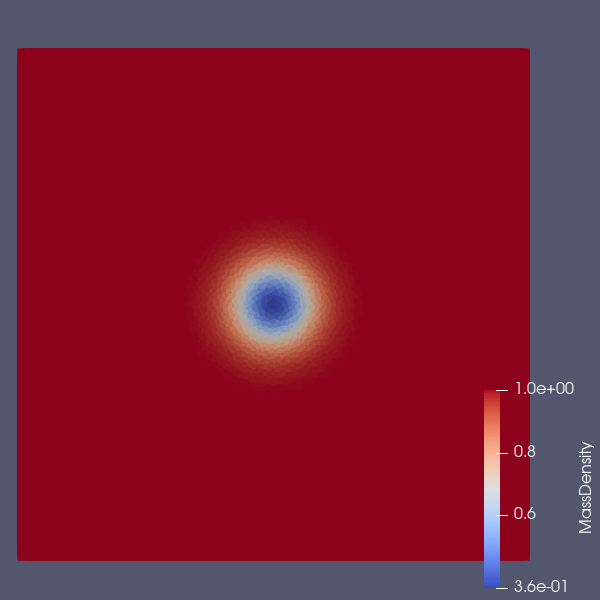
\includegraphics[width=0.47\textwidth]{vortex1.png}
} \hfill
\subcaptionbox{LLS1 reconstruction ($t = 1$).} {
	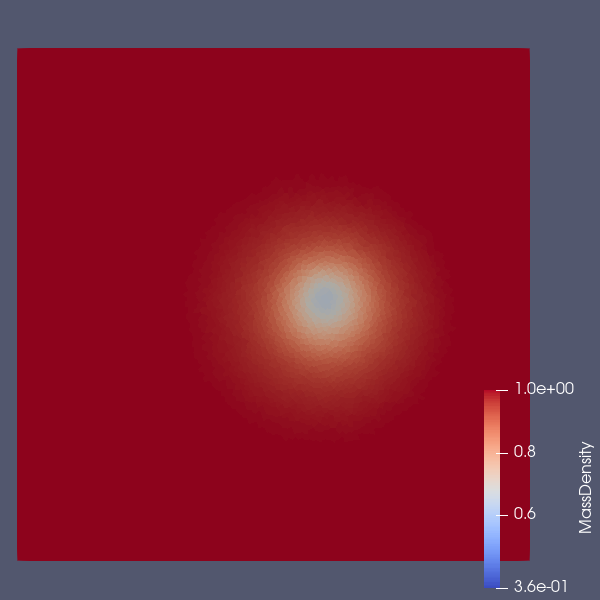
\includegraphics[width=0.47\textwidth]{vortex2.png}
} \\[2em]
\subcaptionbox{LLS2 reconstruction ($t = 1$).} {
	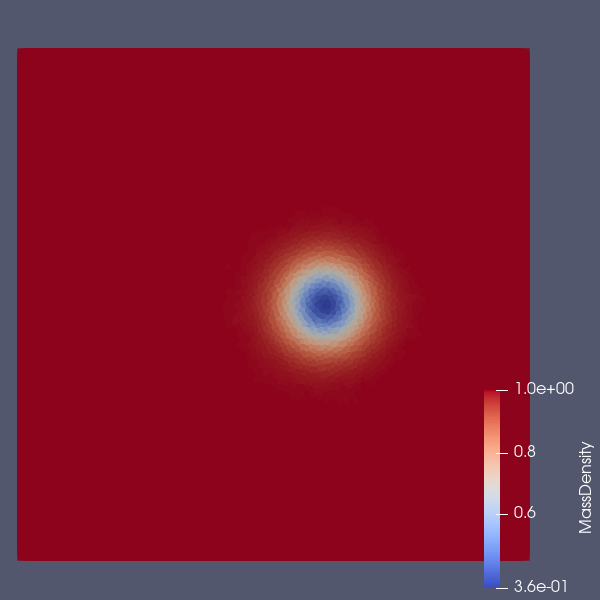
\includegraphics[width=0.47\textwidth]{vortex3.png}
} \hfill
\subcaptionbox{LLS3 reconstruction ($t = 1$).} {
	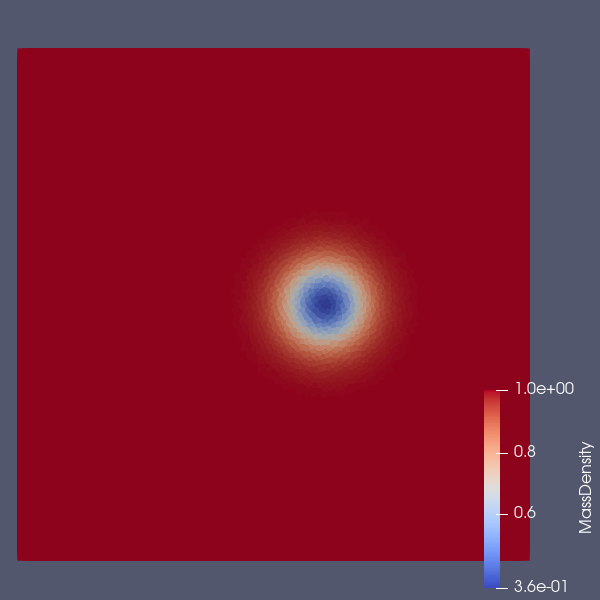
\includegraphics[width=0.47\textwidth]{vortex4.png}
}
\caption{Mass density of the vortex over time.}
\label{fig:comparison-vortex}
\end{figure}

\begin{figure}[p]
\centering
\subcaptionbox{Initial condition ($t = 0$).} {
	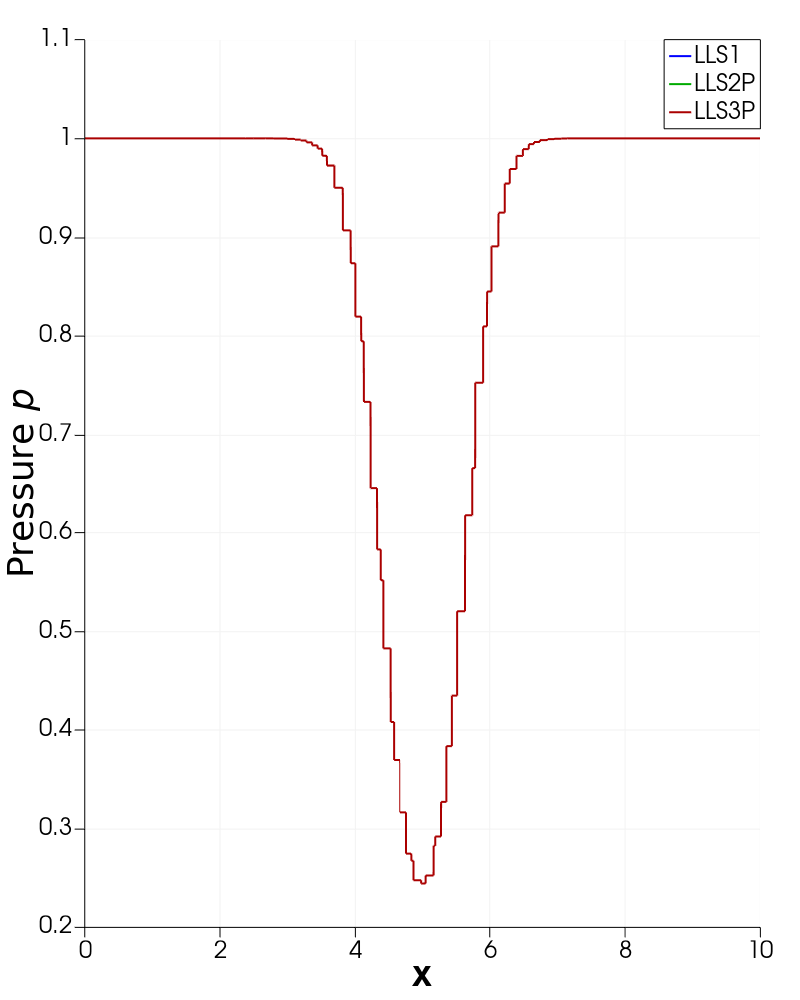
\includegraphics[width=0.47\textwidth]{vortexhor1.png}
} \hfill
\subcaptionbox{Advected vortex ($t = 1$).} {
	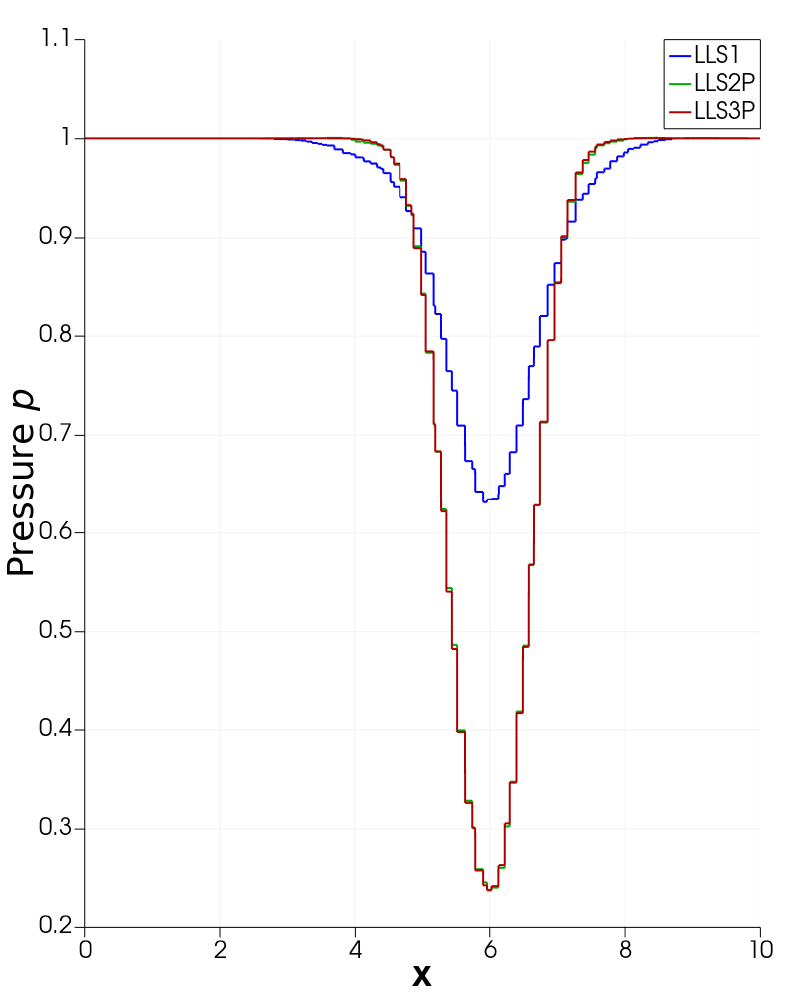
\includegraphics[width=0.47\textwidth]{vortexhor2.png}
}
\caption{Pressure of the vortex over time on the line $y = 0$.}
\label{fig:comparison2-vortex}
\end{figure}

\begin{figure}[p]
\centering
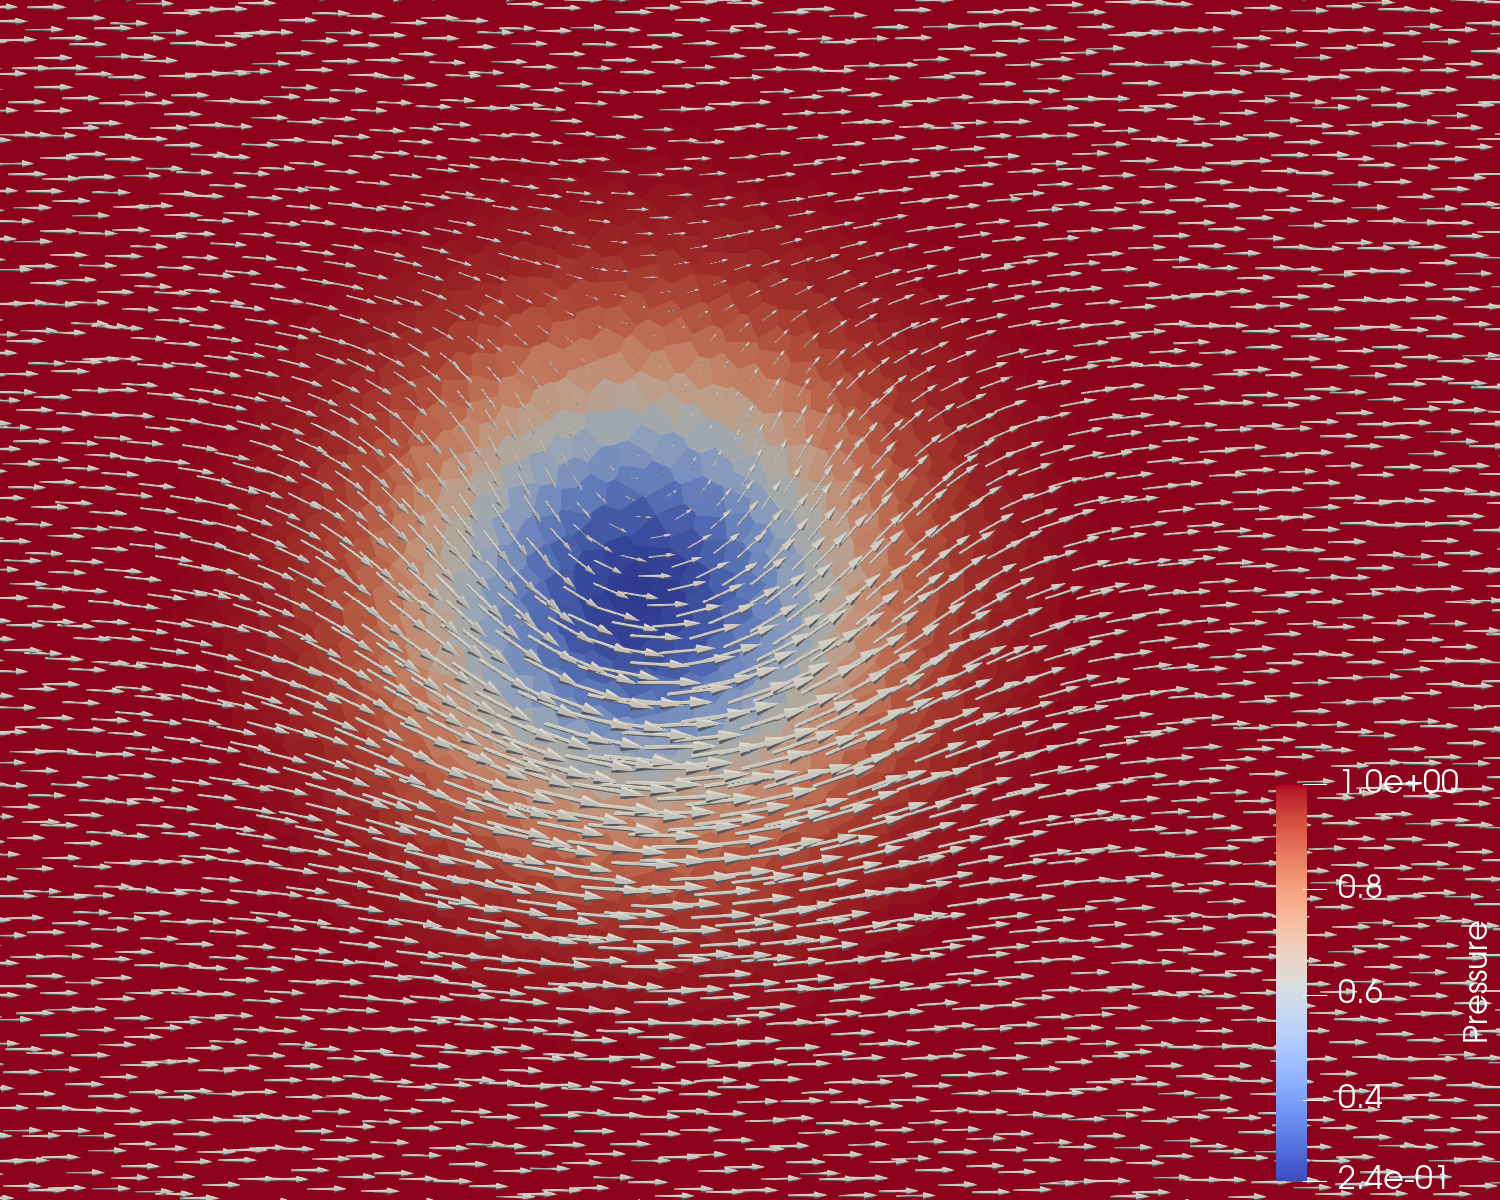
\includegraphics[width=0.9\textwidth]{vortexarrow1.png} \\[2em]
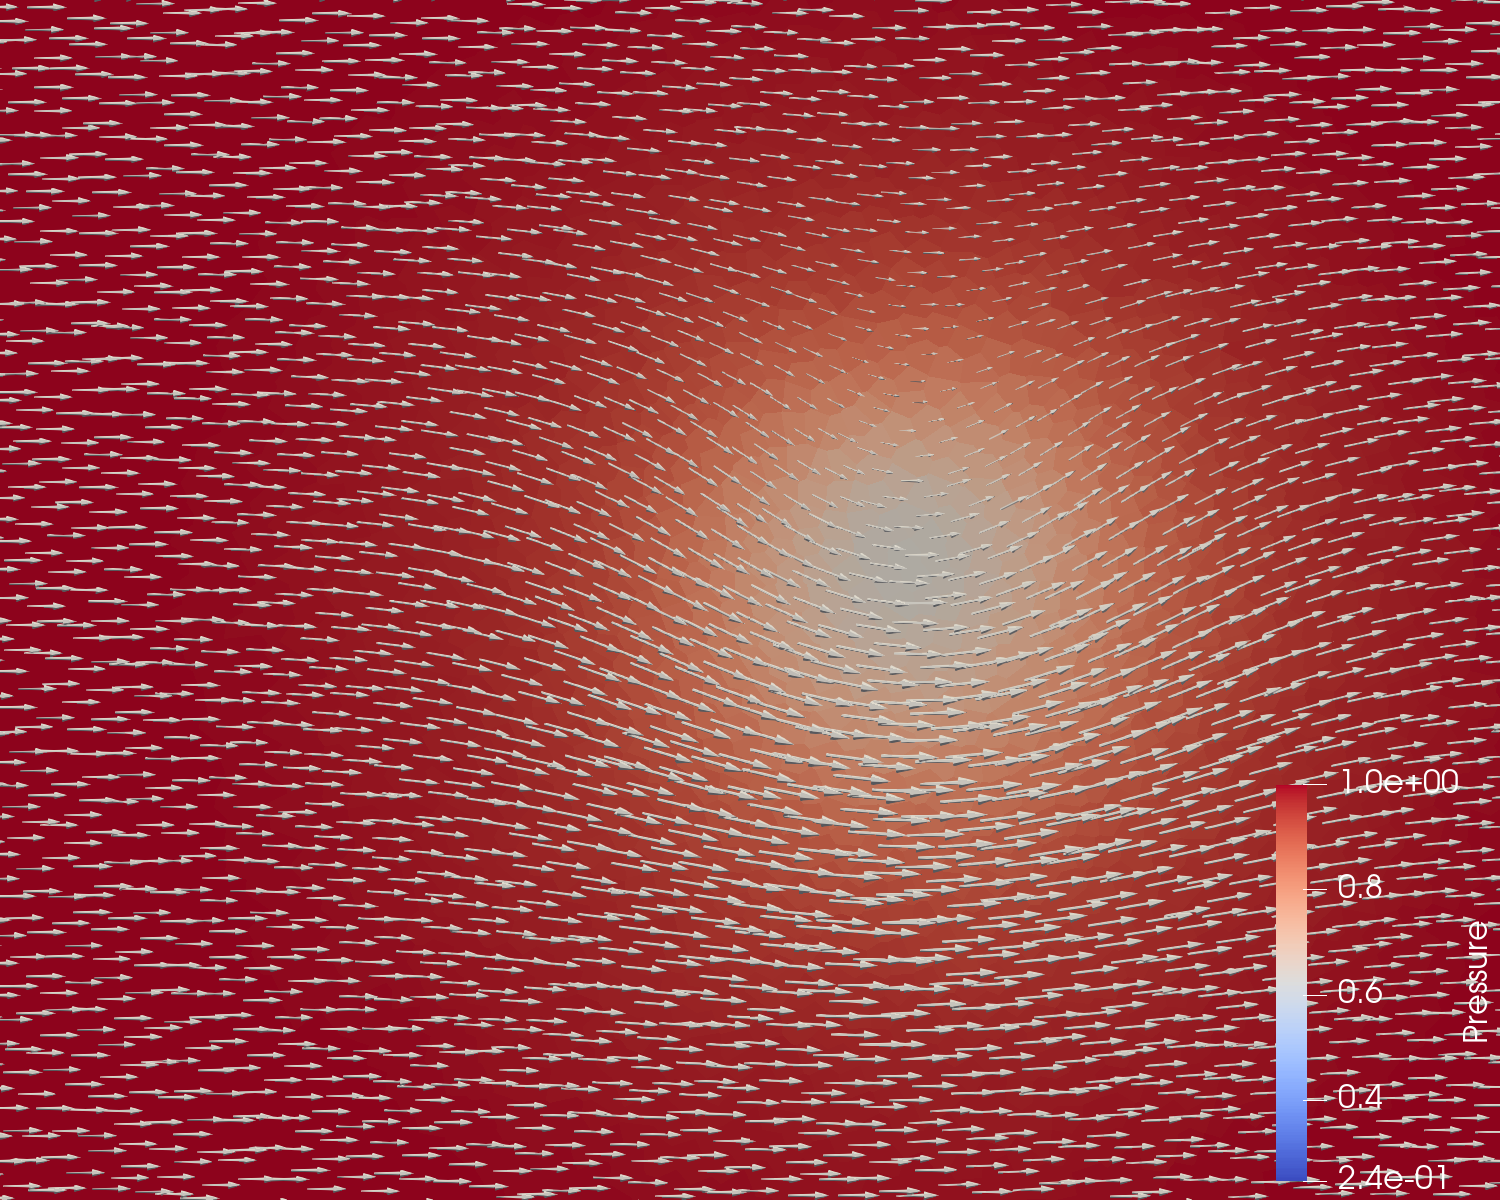
\includegraphics[width=0.9\textwidth]{vortexarrow2.png}
\caption{Attenuation of vortex pressure and velocity by a LLS1 scheme;\\
$t = 0$ above and $t = 1$ below.}
\label{fig:comparison3-vortex}
\end{figure}

\begin{figure}[p]
\centering
\subcaptionbox{Mass density $\rho$.} {
	\begin{tikzpicture}[trim axis left, trim axis right]
	\begin{loglogaxis}[
		xlabel={$h$},
		%ylabel={$L^1$ norm of error on density $\rho$},
		width=0.53\textwidth,
		height=0.4\textheight,
		%ymin=1e-7,
		legend style={anchor=south east,at={(0.975,0.025)}}
	]
	\addplot table[x=h,y=rhoL1] {vortex_regular_LLS1.dat};
	\addplot table[x=h,y=rhoL1] {vortex_regular_LLS2P.dat};
	\addplot table[x=h,y=rhoL1] {vortex_regular_LLS3P.dat};
	\addplot[dashed, domain=0.025:0.2] expression {0.1*x};
	\addplot[dashed, domain=0.025:0.2] expression {0.03*x^2};
	\addplot[dashed, domain=0.025:0.2] expression {0.08*x^3};
	\legend{$\text{LLS1},O(h)$\\$\text{LLS2P},O(h^2)$\\$\text{LLS3P},O(h^3)$\\}
	\end{loglogaxis}
	\end{tikzpicture}
} \hfill
\subcaptionbox{Horizontal momentum $\rho \vec{v}_x$.} {
	\begin{tikzpicture}[trim axis left, trim axis right]
	\begin{loglogaxis}[
		xlabel={$h$},
		%ylabel={$L^1$ norm of error on density $\rho$},
		width=0.53\textwidth,
		height=0.4\textheight,
		%ymin=1e-7,
		legend style={anchor=south east,at={(0.975,0.025)}}
	]
	\addplot table[x=h,y=rhovxL1] {vortex_regular_LLS1.dat};
	\addplot table[x=h,y=rhovxL1] {vortex_regular_LLS2P.dat};
	\addplot table[x=h,y=rhovxL1] {vortex_regular_LLS3P.dat};
	\addplot[dashed, domain=0.025:0.2] expression {0.1*x};
	\addplot[dashed, domain=0.025:0.2] expression {0.08*x^2};
	\addplot[dashed, domain=0.025:0.2] expression {0.2*x^3};
	\legend{$\text{LLS1},O(h)$\\$\text{LLS2P},O(h^2)$\\$\text{LLS3P},O(h^3)$\\}
	\end{loglogaxis}
	\end{tikzpicture}
} \\[2em]
\subcaptionbox{Vertical momentum $\rho \vec{v}_y$.} {
	\begin{tikzpicture}[trim axis left, trim axis right]
	\begin{loglogaxis}[
		xlabel={$h$},
		%ylabel={$L^1$ norm of error on density $\rho$},
		width=0.53\textwidth,
		height=0.4\textheight,
		%ymin=1e-7,
		legend style={anchor=south east,at={(0.975,0.025)}}
	]
	\addplot table[x=h,y=rhovyL1] {vortex_regular_LLS1.dat};
	\addplot table[x=h,y=rhovyL1] {vortex_regular_LLS2P.dat};
	\addplot table[x=h,y=rhovyL1] {vortex_regular_LLS3P.dat};
	\addplot[dashed, domain=0.025:0.2] expression {0.1*x};
	\addplot[dashed, domain=0.025:0.2] expression {0.08*x^2};
	\addplot[dashed, domain=0.025:0.2] expression {0.2*x^3};
	\legend{$\text{LLS1},O(h)$\\$\text{LLS2P},O(h^2)$\\$\text{LLS3P},O(h^3)$\\}
	\end{loglogaxis}
	\end{tikzpicture}
} \hfill
\subcaptionbox{Total energy density $e$.} {
	\begin{tikzpicture}[trim axis left, trim axis right]
	\begin{loglogaxis}[
		xlabel={$h$},
		%ylabel={$L^1$ norm of error on density $\rho$},
		width=0.53\textwidth,
		height=0.4\textheight,
		%ymin=1e-7,
		legend style={anchor=south east,at={(0.975,0.025)}}
	]
	\addplot table[x=h,y=eL1] {vortex_regular_LLS1.dat};
	\addplot table[x=h,y=eL1] {vortex_regular_LLS2P.dat};
	\addplot table[x=h,y=eL1] {vortex_regular_LLS3P.dat};
	\addplot[dashed, domain=0.025:0.2] expression {0.2*x};
	\addplot[dashed, domain=0.025:0.2] expression {0.15*x^2};
	\addplot[dashed, domain=0.025:0.2] expression {0.3*x^3};
	\legend{$\text{LLS1},O(h)$\\$\text{LLS2P},O(h^2)$\\$\text{LLS3P},O(h^3)$\\}
	\end{loglogaxis}
	\end{tikzpicture}
}
\caption{In each plot: $L^1$ norm of the error on the specified
conserved variable.}
\label{fig:comparison-L1-errors-entropy-vortex-regular-grid}
\end{figure}

\begin{figure}[p]
\centering
\subcaptionbox{Mass density $\rho$.} {
	\begin{tikzpicture}[trim axis left, trim axis right]
	\begin{loglogaxis}[
		xlabel={$h$},
		%ylabel={$L^1$ norm of error on density $\rho$},
		width=0.53\textwidth,
		height=0.4\textheight,
		%ymin=1e-7,
		legend style={anchor=south east,at={(0.975,0.025)}}
	]
	\addplot table[x=h,y=rhoLinf] {vortex_regular_LLS1.dat};
	\addplot table[x=h,y=rhoLinf] {vortex_regular_LLS2P.dat};
	\addplot table[x=h,y=rhoLinf] {vortex_regular_LLS3P.dat};
	\addplot[dashed, domain=0.025:0.2] expression {2*x};
	\addplot[dashed, domain=0.025:0.2] expression {0.7*x^2};
	\addplot[dashed, domain=0.025:0.2] expression {3*x^3};
	\legend{$\text{LLS1},O(h)$\\$\text{LLS2P},O(h^2)$\\$\text{LLS3P},O(h^3)$\\}
	\end{loglogaxis}
	\end{tikzpicture}
} \hfill
\subcaptionbox{Horizontal momentum $\rho \vec{v}_x$.} {
	\begin{tikzpicture}[trim axis left, trim axis right]
	\begin{loglogaxis}[
		xlabel={$h$},
		%ylabel={$L^1$ norm of error on density $\rho$},
		width=0.53\textwidth,
		height=0.4\textheight,
		%ymin=1e-7,
		legend style={anchor=south east,at={(0.975,0.025)}}
	]
	\addplot table[x=h,y=rhovxLinf] {vortex_regular_LLS1.dat};
	\addplot table[x=h,y=rhovxLinf] {vortex_regular_LLS2P.dat};
	\addplot table[x=h,y=rhovxLinf] {vortex_regular_LLS3P.dat};
	\addplot[dashed, domain=0.025:0.2] expression {3*x};
	\addplot[dashed, domain=0.025:0.2] expression {1.5*x^2};
	\addplot[dashed, domain=0.025:0.2] expression {7*x^3};
	\legend{$\text{LLS1},O(h)$\\$\text{LLS2P},O(h^2)$\\$\text{LLS3P},O(h^3)$\\}
	\end{loglogaxis}
	\end{tikzpicture}
} \\[2em]
\subcaptionbox{Vertical momentum $\rho \vec{v}_y$.} {
	\begin{tikzpicture}[trim axis left, trim axis right]
	\begin{loglogaxis}[
		xlabel={$h$},
		%ylabel={$L^1$ norm of error on density $\rho$},
		width=0.53\textwidth,
		height=0.4\textheight,
		%ymin=1e-7,
		legend style={anchor=south east,at={(0.975,0.025)}}
	]
	\addplot table[x=h,y=rhovyLinf] {vortex_regular_LLS1.dat};
	\addplot table[x=h,y=rhovyLinf] {vortex_regular_LLS2P.dat};
	\addplot table[x=h,y=rhovyLinf] {vortex_regular_LLS3P.dat};
	\addplot[dashed, domain=0.025:0.2] expression {3*x};
	\addplot[dashed, domain=0.025:0.2] expression {1.5*x^2};
	\addplot[dashed, domain=0.025:0.2] expression {7*x^3};
	\legend{$\text{LLS1},O(h)$\\$\text{LLS2P},O(h^2)$\\$\text{LLS3P},O(h^3)$\\}
	\end{loglogaxis}
	\end{tikzpicture}
} \hfill
\subcaptionbox{Total energy density $e$.} {
	\begin{tikzpicture}[trim axis left, trim axis right]
	\begin{loglogaxis}[
		xlabel={$h$},
		%ylabel={$L^1$ norm of error on density $\rho$},
		width=0.53\textwidth,
		height=0.4\textheight,
		%ymin=1e-7,
		legend style={anchor=south east,at={(0.975,0.025)}}
	]
	\addplot table[x=h,y=eLinf] {vortex_regular_LLS1.dat};
	\addplot table[x=h,y=eLinf] {vortex_regular_LLS2P.dat};
	\addplot table[x=h,y=eLinf] {vortex_regular_LLS3P.dat};
	\addplot[dashed, domain=0.025:0.2] expression {10*x};
	\addplot[dashed, domain=0.025:0.2] expression {5*x^2};
	\addplot[dashed, domain=0.025:0.2] expression {20*x^3};
	\legend{$\text{LLS1},O(h)$\\$\text{LLS2P},O(h^2)$\\$\text{LLS3P},O(h^3)$\\}
	\end{loglogaxis}
	\end{tikzpicture}
}
\caption{In each plot: $L^{\infty}$ norm of the error on the specified
conserved variable.}
\label{fig:comparison-Linf-errors-entropy-vortex-regular-grid}
\end{figure}

%\begin{figure}[p]
%\centering
%\subcaptionbox{$L^1$ norm of the error on a square grid.} {
%	\begin{tikzpicture}[trim axis left, trim axis right]
%	\begin{loglogaxis}[
%		xlabel={$h$},
%		%ylabel={$L^1$ norm of error on density $\rho$},
%		width=0.53\textwidth,
%		height=0.4\textheight,
%		ymin=1e-6, ymax=1e-1,
%		legend style={anchor=south east,at={(0.975,0.025)}}
%	]
%	\addplot table[x=h,y=rhoL1] {waves_regular_LLS1.dat};
%	\addplot table[x=h,y=rhoL1] {waves_regular_LLS2P.dat};
%	\addplot table[x=h,y=rhoL1] {waves_regular_LLS3P.dat};
%	\addplot[dashed, domain=0.025:0.2] expression {0.15*x};
%	\addplot[dashed, domain=0.025:0.2] expression {0.07*x^2};
%	\addplot[dashed, domain=0.025:0.2] expression {0.2*x^3};
%	\legend{$\text{LLS1},O(h)$\\$\text{LLS2P},O(h^2)$\\$\text{LLS3P},O(h^3)$\\}
%	\end{loglogaxis}
%	\end{tikzpicture}
%} \hfill
%\subcaptionbox{$L^1$ norm of the error on a Voronoi grid.} {
%	\begin{tikzpicture}[trim axis left, trim axis right]
%	\begin{loglogaxis}[
%		xlabel={$h$},
%		%ylabel={$L^1$ norm of error on density $\rho$},
%		width=0.53\textwidth,
%		height=0.4\textheight,
%		ymin=1e-6, ymax=1e-1,
%		legend style={anchor=south east,at={(0.975,0.025)}}
%	]
%	\addplot table[x=h,y=rhovxL1] {waves_voronoi_LLS1.dat};
%	\addplot table[x=h,y=rhovxL1] {waves_voronoi_LLS2P.dat};
%	\addplot table[x=h,y=rhovxL1] {waves_voronoi_LLS3P.dat};
%	\addplot[dashed, domain=0.025:0.2] expression {0.15*x};
%	\addplot[dashed, domain=0.025:0.2] expression {0.07*x^2};
%	\addplot[dashed, domain=0.025:0.2] expression {0.2*x^3};
%	\legend{$\text{LLS1},O(h)$\\$\text{LLS2P},O(h^2)$\\$\text{LLS3P},O(h^3)$\\}
%	\end{loglogaxis}
%	\end{tikzpicture}
%} \\[2em]
%\subcaptionbox{$L^{\infty}$ norm of the error on a square grid.} {
%	\begin{tikzpicture}[trim axis left, trim axis right]
%	\begin{loglogaxis}[
%		xlabel={$h$},
%		%ylabel={$L^1$ norm of error on density $\rho$},
%		width=0.53\textwidth,
%		height=0.4\textheight,
%		ymin=1e-6, ymax=1e-1,
%		legend style={anchor=south east,at={(0.975,0.025)}}
%	]
%	\addplot table[x=h,y=rhovyLinf] {waves_regular_LLS1.dat};
%	\addplot table[x=h,y=rhovyLinf] {waves_regular_LLS2P.dat};
%	\addplot table[x=h,y=rhovyLinf] {waves_regular_LLS3P.dat};
%	\addplot[dashed, domain=0.025:0.2] expression {0.25*x};
%	\addplot[dashed, domain=0.025:0.2] expression {0.1*x^2};
%	\addplot[dashed, domain=0.025:0.2] expression {0.4*x^3};
%	\legend{$\text{LLS1},O(h)$\\$\text{LLS2P},O(h^2)$\\$\text{LLS3P},O(h^3)$\\}
%	\end{loglogaxis}
%	\end{tikzpicture}
%} \hfill
%\subcaptionbox{$L^{\infty}$ norm of the error on a Voronoi grid.} {
%	\begin{tikzpicture}[trim axis left, trim axis right]
%	\begin{loglogaxis}[
%		xlabel={$h$},
%		%ylabel={$L^1$ norm of error on density $\rho$},
%		width=0.53\textwidth,
%		height=0.4\textheight,
%		ymin=1e-6, ymax=1e-1,
%		legend style={anchor=south east,at={(0.975,0.025)}}
%	]
%	\addplot table[x=h,y=eLinf] {waves_voronoi_LLS1.dat};
%	\addplot table[x=h,y=eLinf] {waves_voronoi_LLS2P.dat};
%	\addplot table[x=h,y=eLinf] {waves_voronoi_LLS3P.dat};
%	\addplot[dashed, domain=0.025:0.2] expression {0.25*x};
%	\addplot[dashed, domain=0.025:0.2] expression {0.1*x^2};
%	\addplot[dashed, domain=0.025:0.2] expression {0.4*x^3};
%	\legend{$\text{LLS1},O(h)$\\$\text{LLS2P},O(h^2)$\\$\text{LLS3P},O(h^3)$\\}
%	\end{loglogaxis}
%	\end{tikzpicture}
%}
%\caption{Errors in the entropy waves test. All conserved variables give the
%same errors, so only mass density $\rho$ is shown.}
%\label{fig:comparison-errors-entropy-waves}
%\end{figure}































